
\documentclass{article}\usepackage[]{graphicx}\usepackage[]{color}
%% maxwidth is the original width if it is less than linewidth
%% otherwise use linewidth (to make sure the graphics do not exceed the margin)
\makeatletter
\def\maxwidth{ %
  \ifdim\Gin@nat@width>\linewidth
    \linewidth
  \else
    \Gin@nat@width
  \fi
}
\makeatother

\definecolor{fgcolor}{rgb}{0.345, 0.345, 0.345}
\newcommand{\hlnum}[1]{\textcolor[rgb]{0.686,0.059,0.569}{#1}}%
\newcommand{\hlstr}[1]{\textcolor[rgb]{0.192,0.494,0.8}{#1}}%
\newcommand{\hlcom}[1]{\textcolor[rgb]{0.678,0.584,0.686}{\textit{#1}}}%
\newcommand{\hlopt}[1]{\textcolor[rgb]{0,0,0}{#1}}%
\newcommand{\hlstd}[1]{\textcolor[rgb]{0.345,0.345,0.345}{#1}}%
\newcommand{\hlkwa}[1]{\textcolor[rgb]{0.161,0.373,0.58}{\textbf{#1}}}%
\newcommand{\hlkwb}[1]{\textcolor[rgb]{0.69,0.353,0.396}{#1}}%
\newcommand{\hlkwc}[1]{\textcolor[rgb]{0.333,0.667,0.333}{#1}}%
\newcommand{\hlkwd}[1]{\textcolor[rgb]{0.737,0.353,0.396}{\textbf{#1}}}%
\let\hlipl\hlkwb

\usepackage{framed}
\makeatletter
\newenvironment{kframe}{%
 \def\at@end@of@kframe{}%
 \ifinner\ifhmode%
  \def\at@end@of@kframe{\end{minipage}}%
  \begin{minipage}{\columnwidth}%
 \fi\fi%
 \def\FrameCommand##1{\hskip\@totalleftmargin \hskip-\fboxsep
 \colorbox{shadecolor}{##1}\hskip-\fboxsep
     % There is no \\@totalrightmargin, so:
     \hskip-\linewidth \hskip-\@totalleftmargin \hskip\columnwidth}%
 \MakeFramed {\advance\hsize-\width
   \@totalleftmargin\z@ \linewidth\hsize
   \@setminipage}}%
 {\par\unskip\endMakeFramed%
 \at@end@of@kframe}
\makeatother

\definecolor{shadecolor}{rgb}{.97, .97, .97}
\definecolor{messagecolor}{rgb}{0, 0, 0}
\definecolor{warningcolor}{rgb}{1, 0, 1}
\definecolor{errorcolor}{rgb}{1, 0, 0}
\newenvironment{knitrout}{}{} % an empty environment to be redefined in TeX

\usepackage{alltt}

\usepackage{natbib}
\usepackage{graphics}
\usepackage{amsmath}
\usepackage{indentfirst}
\usepackage[utf8]{inputenc}
\usepackage{color}
\usepackage{hyperref}
\IfFileExists{upquote.sty}{\usepackage{upquote}}{}
\begin{document}
%\SweaveOpts{concordance=TRUE}
\title{rnaCleanR: an R package to quantify and remove putative DNA contamination from strand specific RNA-seq}
\author{Thu-Hien To & Steve Pederson}
\maketitle

\tableofcontents

\clearpage

\section{Introduction}

\textit{rnaCleanR} is a package used to quantify and remove double-strand DNA within a strand-specific RNA-seq. It takes as input one or several bam files and uses a window sliding across each chromosome. For each window, it considers the proportion of positive/negative reads comparing to a given threshold, to suggest that  windows contains single strand RNA or double strand DNA. Then each read fragment is assigned to a probability of being kept or not, based on the proportion of positive/negative of the windows that contain that fragment.

The input bam file must be sorted and an index file must be given at the same folder. The average read length is required to calculate the size of sliding window and its step. 


\section{Get plots}

The function \textit{getPlot} can be used to get some plots on the amount of positive/negative reads over all windows. You can also have these plots at the same time as filtering the bam file by using function \textit{filterOne} with options \textit{histPlot=TRUE} or \textit{winPlot=TRUE}.


\begin{knitrout}
\definecolor{shadecolor}{rgb}{0.969, 0.969, 0.969}\color{fgcolor}\begin{kframe}
\begin{alltt}
\hlkwd{library}\hlstd{(rnaCleanR)}
\hlstd{file} \hlkwb{<-} \hlkwd{system.file}\hlstd{(}\hlstr{"data"}\hlstd{,}\hlstr{"s1.chr1.bam"}\hlstd{,}\hlkwc{package} \hlstd{=} \hlstr{"rnaCleanR"}\hlstd{)}
\hlkwd{getPlot}\hlstd{(}\hlkwc{bamfilein} \hlstd{= file,}\hlkwc{readLength} \hlstd{=} \hlnum{100}\hlstd{,}\hlkwc{histPlotFile} \hlstd{=} \hlstr{"hist.pdf"}\hlstd{,}
        \hlkwc{winPlotFile} \hlstd{=} \hlstr{"win.pdf"}\hlstd{)}
\end{alltt}
\end{kframe}
\end{knitrout}


Two figures \textit{hist.pdf} and \textit{win.pdf} will be created.

\textit{hist.pdf} (Fig. \ref{fig:hist}) is a histogram on the frequency of positive proportion over all windows, which give you an idea on how much double-strand DNA is contained in your sample. We split it into $4$ catergories based on the maximum coverage of the window: smaller than $10$, from $10$ to $100$, from $100$ to $1000$ and above $1000$. In perfectly clear ss-RNA-seq, the positive proportion of every window should be either around 0$\%$ or 100$\%$. The more amount of windows have this proportion around 50$\%$, the more your sample is DNA contaminated.

\begin{figure}[H]
  \centering
  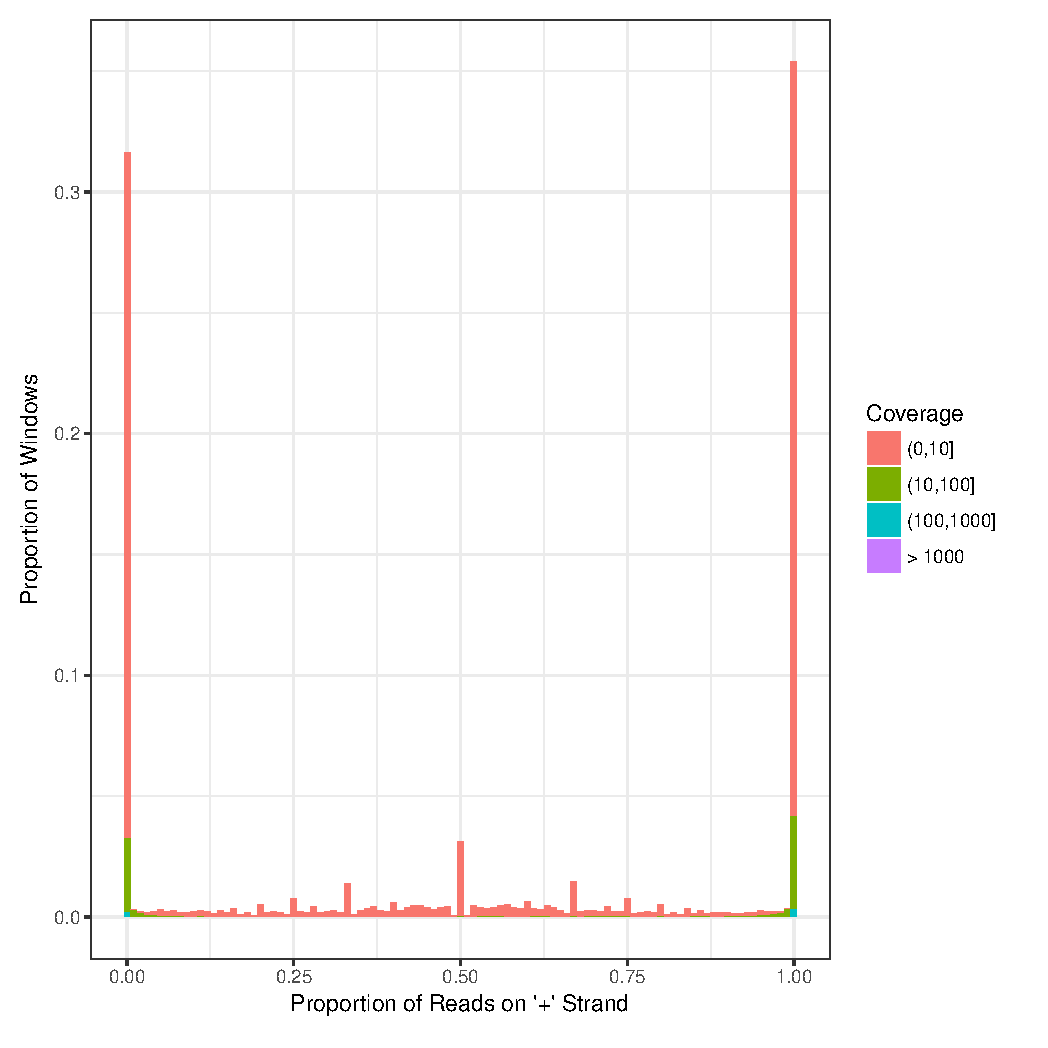
\includegraphics[width=\maxwidth]{hist.pdf}
  \caption{Histogram of positive proportion across all windows.}
  \label{fig:hist}
\end{figure}

\textif{win.pdf} (Fig. \ref{fig:win}) is a plot on the number of reads vs positive proportion within each window. There are also $4$ lines correspond to $4$ representative thresholds ($0.6$, $0.7$, $0.8$, $0.9$). Threshold is a parameter that the user should give for filtering a bam file. 
Given a threshold, a positive (resp. negative) window is kept if and only if it is above (resp. below) the corresponding threshold line on this plot. Looking at this plot, we can have an idea of which threshold to be used for filtering DNA from your sample. The windows are also breaken down in $4$ groups based on its maximum coverage.

\begin{figure}[H]
  \centering
  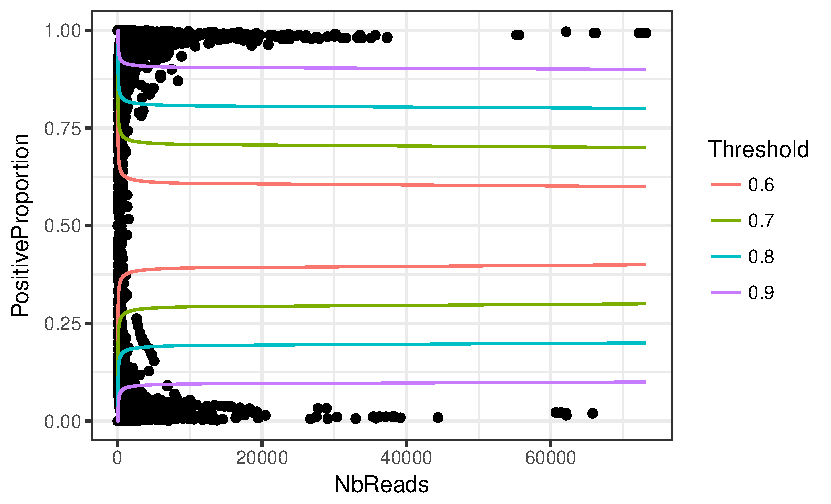
\includegraphics[width=\maxwidth]{win.pdf}
  \caption{Sum of reads vs positive proportion across all windows.}
  \label{fig:win}
\end{figure}

\section{Filter bam files}

The functions \textit{filterOne} removes potential double strand DNA from one bam file, while \textit{filterMulti} filters several bam files. The later method uses the merged alignments from all input bam files to decide which windows are kept; then each individual bam file is filtered based on the same set of kept windows.

To filter one bamfile:

\begin{knitrout}
\definecolor{shadecolor}{rgb}{0.969, 0.969, 0.969}\color{fgcolor}\begin{kframe}
\begin{alltt}
\hlstd{file} \hlkwb{<-} \hlkwd{system.file}\hlstd{(}\hlstr{"data"}\hlstd{,}\hlstr{"s1.chr1.bam"}\hlstd{,}\hlkwc{package} \hlstd{=} \hlstr{"rnaCleanR"}\hlstd{)}
\hlkwd{filterOne}\hlstd{(}\hlkwc{bamfilein} \hlstd{= file,}\hlkwc{bamfileout} \hlstd{=} \hlstr{"filter.bam"}\hlstd{,}
          \hlkwc{readLength} \hlstd{=} \hlnum{100}\hlstd{,} \hlkwc{threshold} \hlstd{=} \hlnum{0.7}\hlstd{)}
\end{alltt}
\end{kframe}
\end{knitrout}

Other parameters can be specified for more flexible filtering: define the ranges that you want to always keep, the min coverage that you want to ignore, the rate that an RNA read has false strand etc. Further information can be found in the manual page of the function accessible from (\textit{?filterOne}).


If you want to get plots at the same time as filtering, then:

\begin{knitrout}
\definecolor{shadecolor}{rgb}{0.969, 0.969, 0.969}\color{fgcolor}\begin{kframe}
\begin{alltt}
\hlkwd{filterOne}\hlstd{(}\hlkwc{bamfilein} \hlstd{= file,}\hlkwc{bamfileout} \hlstd{=} \hlstr{"filter.bam"}\hlstd{,}
          \hlkwc{readLength} \hlstd{=} \hlnum{100}\hlstd{,} \hlkwc{threshold} \hlstd{=} \hlnum{0.7}\hlstd{,}\hlkwc{histPlot} \hlstd{=} \hlnum{TRUE}\hlstd{,}
          \hlkwc{histPlotFile} \hlstd{=} \hlstr{"hist.pdf"}\hlstd{,}\hlkwc{winPlot} \hlstd{=} \hlnum{TRUE}\hlstd{,}\hlkwc{winPlotFile} \hlstd{=} \hlstr{"win.pdf"}\hlstd{)}
\end{alltt}
\end{kframe}
\end{knitrout}


Finally is an example for filtering 2 bam files.

\begin{knitrout}
\definecolor{shadecolor}{rgb}{0.969, 0.969, 0.969}\color{fgcolor}\begin{kframe}
\begin{alltt}
\hlstd{file} \hlkwb{<-} \hlkwd{system.file}\hlstd{(}\hlstr{"data"}\hlstd{,}\hlkwd{c}\hlstd{(}\hlstr{"s1.chr1.bam"}\hlstd{,}\hlstr{"s2.chr1.bam"}\hlstd{),}\hlkwc{package} \hlstd{=} \hlstr{"rnaCleanR"}\hlstd{)}
\hlkwd{filterMulti}\hlstd{(}\hlkwc{bamfilein} \hlstd{= file,}\hlkwc{bamfileout} \hlstd{=} \hlkwd{c}\hlstd{(}\hlstr{"filter1.bam"}\hlstd{,}\hlstr{"filter2.bam"}\hlstd{),}
            \hlkwc{readLength} \hlstd{=} \hlnum{100}\hlstd{,} \hlkwc{threshold} \hlstd{=} \hlnum{0.7}\hlstd{)}
\end{alltt}
\end{kframe}
\end{knitrout}

\end{document}
